\let\negmedspace\undefined
\let\negthickspace\undefined
\documentclass[journal]{IEEEtran}
\usepackage[a5paper, margin=10mm, onecolumn]{geometry}
%\usepackage{lmodern} % Ensure lmodern is loaded for pdflatex
\usepackage{tfrupee} % Include tfrupee package

\setlength{\headheight}{1cm} % Set the height of the header box
\setlength{\headsep}{0mm}     % Set the distance between the header box and the top of the text

\usepackage{gvv-book}
\usepackage{gvv}
\usepackage{cite}
\usepackage{amsmath,amssymb,amsfonts,amsthm}
\usepackage{algorithmic}
\usepackage{graphicx}
\usepackage{textcomp}
\usepackage{xcolor}
\usepackage{txfonts}
\usepackage{listings}
\usepackage{enumitem}
\usepackage{mathtools}
\usepackage{gensymb}
\usepackage{comment}
\usepackage[breaklinks=true]{hyperref}
\usepackage{tkz-euclide} 
\usepackage{listings}
\usepackage{tikz}
\usetikzlibrary{patterns}
% \usepackage{gvv}                                        
\def\inputGnumericTable{}                                 
\usepackage[latin1]{inputenc}                                
\usepackage{color}                                            
\usepackage{array}                                            
\usepackage{longtable}                                       
\usepackage{calc}                                             
\usepackage{multirow}                                         
\usepackage{hhline}                                           
\usepackage{ifthen}                                           
\usepackage{lscape}
\usepackage{multicol}
\begin{document}

\bibliographystyle{IEEEtran}
\vspace{3cm}

\title{AE : Aerospace Engineering}
\author{AI24BTECH11022 - Pabbuleti Venkata Charan Teja}
\maketitle

\renewcommand{\thefigure}{\theenumi}
\renewcommand{\thetable}{\theenumi}


\begin{enumerate}
\setcounter{enumi}{52}
\item In the figure shown below, the magnitude of internal force in member $BC$
is \rule{1cm}{0.15mm} $N$ (rounded off to $1$ decimal place).

\begin{tikzpicture}[scale=0.75]
\def\radius{2}
\def\smallradius{1.414}
\foreach \angle [count=\i] in {0,45,...,315} {
\coordinate (A\i) at (\angle+22.5:\radius);
}
\foreach \i [remember=\i as \lasti (initially 8)] in {7} {
\fill[gray!30] (0,0) -- (A\i) -- (A\lasti) -- cycle;
}
\foreach \i [remember=\i as \lasti (initially 5)] in {4,3} {
\fill[gray!30] (0,0) -- (A\i) -- (A\lasti) -- cycle;
}

\foreach \i [remember=\i as \lasti (initially 8)] in {1,...,8} {
\draw (A\lasti) -- (A\i);
}
\begin{scope}[shift={(2.2,-2.2)}]
\foreach \angle [count=\i] in {0,60,...,300} {
\coordinate (B\i) at (\angle+45:\smallradius);
}
\foreach \i [remember=\i as \lasti (initially 6)] in {1,2} {
\fill[gray!30] (0,0) -- (B\i) -- (B\lasti) -- cycle;
}
\foreach \i [remember=\i as \lasti (initially 6)] in {1,...,6} {
\draw (B\lasti) -- (B\i);
}
\end{scope}
\draw[dashed,thick] (4,-4) -- (4,2.5);
\end{tikzpicture}


\item The cross section of a thin-walled beam with uniform wall thickness $t$, shown in the figure, is subjected to a bending moment $M_{x}=10Nm$. If $h=1m$ and $t=0.001m$, the magnitude of maximum normal stress in the cross section is \rule{1cm}{0.15mm} $N/m^{2}$ (answer in integer).

\begin{circuitikz}
\draw (5,0) to [R=$2\ohm$] (3,0) to [closing switch, l=S] (2,0) to [battery1,l=$10V$] (0,0) -- (0,1) to [C=$1\micro F$] (2.5,1) to [R=$10\ohm$] (5,1);
\draw (4,3) -- (5,3) -- (5,0);
\draw (0,0) -- (0,3) -- (1,3) -- (1,3.5) to [R=$6\ohm$] (4,3.5) -- (4,2.5) to [R=$3\ohm$] (1,2.5) -- (1,3);
\end{circuitikz}

\item The equations of motion for a two degrees of freedom undamped spring-mass system are : $$mx_{1}+2kx_{1}-kx_{2}=0$$ $$mx_{2}-kx_{1}+2kx_{2}=0$$ where $m$ and $k$ represent mass and stiffness respectively, in corresponding SI units, and $x_{1}$ and $x_{2}$ are the degrees of freedom. The larger of the two natural frequencies is given by: $\omega=\alpha\sqrt{\frac{k}{m}}rad/s$. The value of $\alpha$ is \rule{1cm}{0.15mm} (rounded off to 2 decimal places).


\item Consider the plane strain field given by $$\epsilon_{xx}=10xy^{2},\epsilon_{yy}=-5x^{2}y\text{ and }\gamma_{xy}=Axy\brak{2x-y}$$ where, $A$ is a constant and $\gamma_{xy}$ is the engineering shear strain. The value of the constant $A$ for the strain field to be compatible is \rule{1cm}{0.15mm} (rounded off to $1$ decimal place).


\item A chemical rocket with an ideally expanded flow through the nozzle produces $5\times 10^{6}N$ thrust at sea level. The specific impulse of the rocket is $200s$ and acceleration due to gravity at the sea level is $9.8m/s^{2}$. The propellent mass flow rate out of the rocket nozzle is \rule{1cm}{0.15mm} $kg/s$ (rounded off to the nearest integer).


\item A centrifugal compressor is designed to operate with air. At the leading edge of the tip of the inducer (eye of the impeller), the blade angle is $45\degree$, and the relative Mach number is $1.0$. The stagnation temperature of the incoming air is $300K$. Consider $\gamma=1.4$. Neglect pre-whirl and slip. The inducer tip speed is \rule{1cm}{0.15mm} $m/s$ (rounded off to the nearest integer).


\item Consider the following Fanno flow problem: Flow enters a constant area duct at a temperature of $273K$ and a Mach number $0.2$ and eventually reaches sonic condition (Mach number $=1$) due to friction. Assume $\gamma=1.4$. The static temperature at the location where sonic condition is reached is \rule{1cm}{0.15mm} $K$ (rounded off to $2$ decimal places).


\item Consider an artificial satellite moving around the Moon in an elliptic orbit. The altitude of the satellite from the Moon's surface at the perigee is $25km$ and that at the apogee is $134km$. Assume the Moon to be spherical with a radius of $1737km$. The trajectory is considered with reference to a coordinate system fixed to the center of mass of the Moon. The ratio of the speed of the satellite at the perigee to that at the apogee is \rule{1cm}{0.15mm} (rounded off to $2$ decimal places).


\item For an aircraft moving at $4km$ altitude above mean sea level at a Mach number of $0.2$, the ratio of equivalent air speed to true air speed is \rule{1cm}{0.15mm} (rounded off to $2$ decimal places).\\

The density of air at mean sea level is $1.225kg/m^{3}$ and at $4km$ altitude is $0.819kg/m^{3}$.


\item For a general aviation airplane, one of the complex conjugate pair of eigenvalues for longitudinal dynamics is given by $-0.039\pm 0.0567i$ (in SI units). If the system is disturbed to excite only this mode, the time taken for the amplitude of response to become half in magnitude is \rule{1cm}{0.15mm} $s$ (rounded off to $1$ decimal place).


\item The figure (not to scale) shows a control volume to estimate the forces on the airfoil with elliptic cross-section. Surfaces $2$ and $3$ are streamlines. Velocity profiles are measured at the upstream end (surface $1$) and at the downstream end (surface $4$) of the control volume. The drag coefficient for the airfoil is defined as $C_{d}=\frac{D}{\frac{1}{2}\rho U_{\infty}^{2}c}$, where $D$ is the drag force on the airfoil per unit span and $\rho$ is the density of the air. The static pressure, $p_{\infty}$, is constant over the entire surface of the control volume. Assuming the flow to be incompressible, two-dimensional and steady, the $C_{d}$ for the airfoil is \rule{1cm}{0.15mm} (rounded off to $3$ decimal places).

\begin{tikzpicture}
\foreach \x in {-2,-1,0,1,2} {
\draw[->] (0,\x/2) -- (1,\x/2);
}
\draw[<->] (-0.2,-1) -- (-0.2,0) node[midway,left] {$H_{U}$};
\draw[<->] (-0.2,1) -- (-0.2,0) node[midway,left] {$H_{U}$};
\node at (0.5,1.25) {$u=U_{\infty}$};
\draw[dashed] (1,-0.5) -- (1,1);
\draw (1,-0.75) circle (0.2cm);
\node at (1,-0.75) {$1$};
\draw[->] (1.1,0) -- (1.75,0) node[right] {$x$};
\draw[->] (1.1,0) -- (1.1,0.75) node[right] {$y$};
\draw[dashed] (1,1) parabola (1.25,1.25);
\draw[dashed] (1,-1) parabola (1.25,-1.25);
\draw[dashed] plot[smooth,domain=1:2] ({\x^2+0.25},\x+0.25);
\draw[dashed] plot[smooth,domain=1:2] ({\x^2+0.25},-\x-0.25);
\draw (4.45,2.25) circle (0.2cm);
\node at (4.45,2.25) {$3$};
\draw (4.45,-2.25) circle (0.2cm);
\node at (4.45,-2.25) {$2$};
\draw[dashed] plot[smooth,domain=2.1:2.5] ({\x^2+0.25},\x+0.25);
\draw[dashed] plot[smooth,domain=2.1:2.5] ({\x^2+0.25},-\x-0.25);
\draw[dashed] (6.5,2.75) -- (9,2.75);
\draw[dashed] (6.5,-2.75) -- (9,-2.75);
\draw[<->] (8.75,0) -- (8.75,2.75) node[midway,left] {$H_{D}=0.03c$};
\draw[<->] (8.75,0) -- (8.75,-2.75) node[midway,left] {$H_{D}=0.03c$};
\draw[dashed] (9.25,-2.15) -- (9.25,2.75);
\draw[dashed] (9.25,-2.75) -- (9.25,-2.55);
\draw (9.25,-2.35) circle (0.2cm);
\node at (9.25,-2.35) {$4$};
\draw (10,2.75) -- (9.25,0) node[midway,right] {$u=\brak{y/H_{D}}U_{\infty}$} -- (10,-2.75) node[midway,right] {$u=\brak{-y/H_{D}}U_{\infty}$};
\draw[->] (9.25,-2.75) -- (10,-2.75);
\draw[->] (9.25,-2) -- (9.8,-2);
\draw[->] (9.25,-1.25) -- (9.6,-1.25);
\draw[->] (9.25,2.75) -- (10,2.75);
\draw[->] (9.25,2) -- (9.8,2);
\draw[->] (9.25,1.25) -- (9.6,1.25);
\node at (6.5,3) {streamline};
\node at (6.5,-3) {streamline};
\draw[<->] (3,-0.5) -- (5,-0.5) node[midway,above] {$c$};
\draw (4,0) ellipse (1cm and 0.15cm);
\end{tikzpicture}


\item An airplane of mass $1000kg$ is in a steady level flight with a speed of $50m/s$. The wing has an elliptic planform with a span of $20m$ and planform area $31.4m^{2}$. Assuming the density of air at that altitude to be $1kg/m^{3}$ and acceleration due to gravity to be $10m/s^{2}$, the induced drag on the wing is \rule{1cm}{0.15mm} $N$ (rounded off to $1$ decimal place).


\item It is desired to estimate the aerodynamic drag, $D$, on a car traveling at a speed of $30m/s$. A one-third scale model of the car is tested in a wind-tunnel following the principles of dynamic similarity. The drag on the scaled model is measured to be $D_{m}$. The ratio $D/D_{m}$ is \rule{1cm}{0.15mm} (rounded off to $1$ decimal place).
\end{enumerate}
\end{document}